\section{Results}
In this section, we compare our results using PDT with the ones computed using
ONELD\cite{cepxs}. PDT is a three dimensional Parallel Deterministic Transport code developed at
Texas A\&M University while ONELD is a code that solves the  
equation (\ref{solved}) in one dimension using the cross sections generated by CEPXS. 
To compare the results produced by the two codes, we use equivalent angular 
discretization, Gauss-Legendre for ONELD, and Gauss-Legendre-Chebyshevv(GLC) for our
code. The GLC quadrature consists of a Gauss-Legendre
quadrature for the polar angle and a Chebyshev quadrature for the azimuthal
angle. The $n$-points Chebyshev quadrature uses $n$ points equally spaced
between 0 and $2\pi$. When the solution is independent of the azimuthal angle,
the GLC quadrature is equivalent to the one dimensional Gauss-Legendre
quadrature. The results of ONELD gives only the average dose on a cell while
the results of our code gives the dose at a given point. To compare the dose
at any given point, we have interpolated the values given by ONELD.

%\subsection{Water}
%Here, we use a $S_{12}$ quadrature. The medium is 5 cm thick and there is an 
%incoming flux of photons. The direction of the flux is chosen to be the most 
%normal direction of the quadrature and the value of the flux on the boundary is 1 
%$\frac{photon}{cm^2s}$. The source of photons has an energy of 20 MeV and we use 
%a cut-off energy of 0.01 MeV. Every particle that has an energy lower than 
%0.01 MeV is assumed to deposit all its energy without moving further.\\
%In the next table, we show the dose computed every centimeter using a
%different scattering \hbox{order :}
%\begin{table}[H]
%\begin{center}
%\caption{Dose in $\frac{MeV}{g}$ for different scattering orders}
%\begin{tabular}{|c|c|c|c|c|c|c|}
%\hline
%Position & ONELD & order = 13 & order = 11 & order = 9 & order = 7 & order = 5 \\
%\hline
%0 & 4.92645e-3 &  &  &  & 6.99349e-3 &  \\
%1 & 5.68274e-2 &  &  &  & 5.36101e-2 &  \\
%2 & 1.05076e-1 &  &  &  & 1.04073e-1 &  \\
%3 & 1.47528e-1 &  &  &  & 1.47958e-1 &  \\
%4 & 1.82864e-1 &  &  &  & 1.81629e-1 &  \\
%5 & 1.85907e-1 &  &  &  & 1.56533e-1 &  \\
%\hline
%\end{tabular}
%\end{center}
%\end{table}     

\subsection{Aluminium}
The setup of this problem, is the same as that of the previous one except now 
the medium is composed of aluminium. In the following table, we show the dose 
computed every centimeter using a different scattering order :
\begin{table}[H]
\begin{center}
\caption{Dose in $\frac{MeV}{g}$ for different scattering orders}
\begin{tabular}{|c|c|c|c|c|c|c|}
\hline
Position & ONELD & order = 13 & order = 11 & order = 9 & order = 7 & order = 5 \\
\hline
0 & 0.015003 & 0.0146404 & 0.0146402 & 0.0141156 & 0.0166718 & 0.0087276 \\
1 & 0.169908 & 0.1697907 & 0.1697890 & 0.1698012 & 0.1695422 & 0.1728969 \\
2 & 0.275425 & 0.2752749 & 0.2752729 & 0.2753298 & 0.2742052 & 0.2775113 \\
3 & 0.316307 & 0.3161310 & 0.3161307 & 0.3165279 & 0.3145572 & 0.3199176 \\
4 & 0.312283 & 0.3120572 & 0.3120566 & 0.3125514 & 0.3104412 & 0.3153226 \\
5 & 0.233048 & 0.2087631 & 0.2087634 & 0.2094064 & 0.2061794 & 0.2154810 \\
\hline
\end{tabular}
\end{center}
\end{table}     
The agreement between ONELD and our code using the full order is excellent.
The differences on the edges of the domain are larger, due to the fact that
the dose varies quickly near the border. Because of this, the interpolation 
used to find the value at a given point by ONELD is not very accurate.\\ 
We see that if we discard the results on the edges of the domain, the results 
obtained by using a $P_5$ order for the scattering are very close to the ones 
using the
full order in the scattering cross-section expansion. The reason is that the 
high order flux moments are very small. Below,
we show several flux moments for different groups. The abscissa is the distance in
centimeters and the ordinate is the value of the flux in $\frac{particles}{cm^2
s}$.
\begin{figure}[H]
\begin{minipage}[b]{0.42\linewidth}
\centering
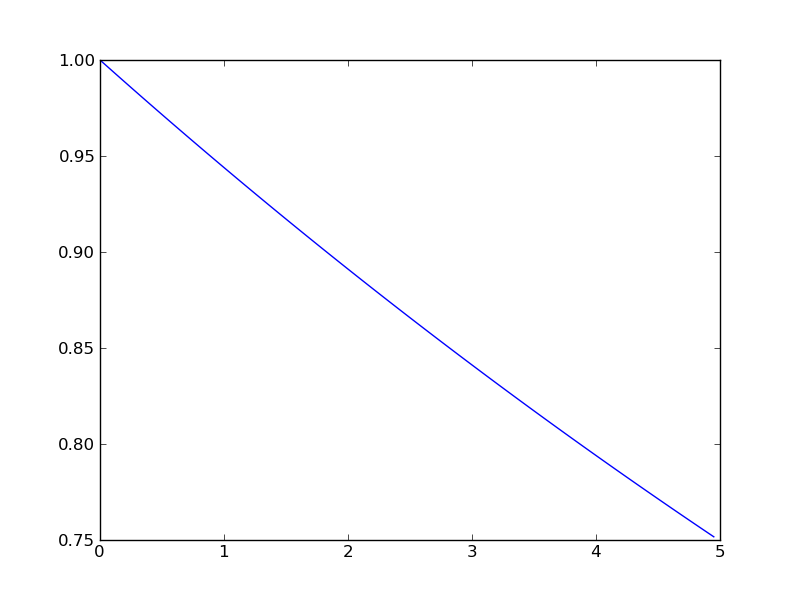
\includegraphics[width=\linewidth]{./images/al/group_0_moment_0}
\caption{Scalar flux in the first photon group}
\end{minipage}
\hspace{0.5cm}
\begin{minipage}[b]{0.42\linewidth}
\centering
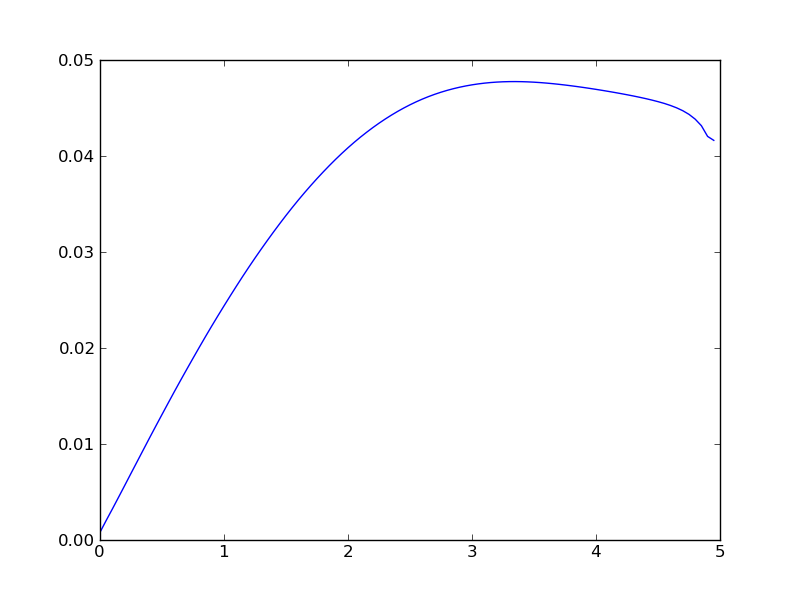
\includegraphics[width=\linewidth]{./images/al/group_39_moment_0}
\caption{Scalar flux in the last electron group}
\end{minipage}
\end{figure}

\begin{figure}[H]
\begin{minipage}[b]{0.42\linewidth}
\centering
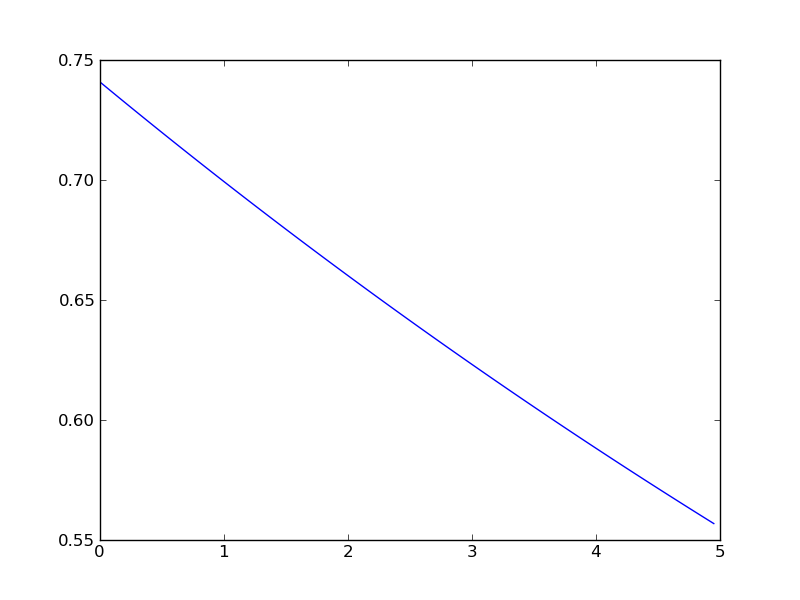
\includegraphics[width=\linewidth]{./images/al/group_0_moment_30}
\caption{Moment $P_5^0$ of the flux in the first photon group}
\end{minipage}
\hspace{0.5cm}
\begin{minipage}[b]{0.42\linewidth}
\centering
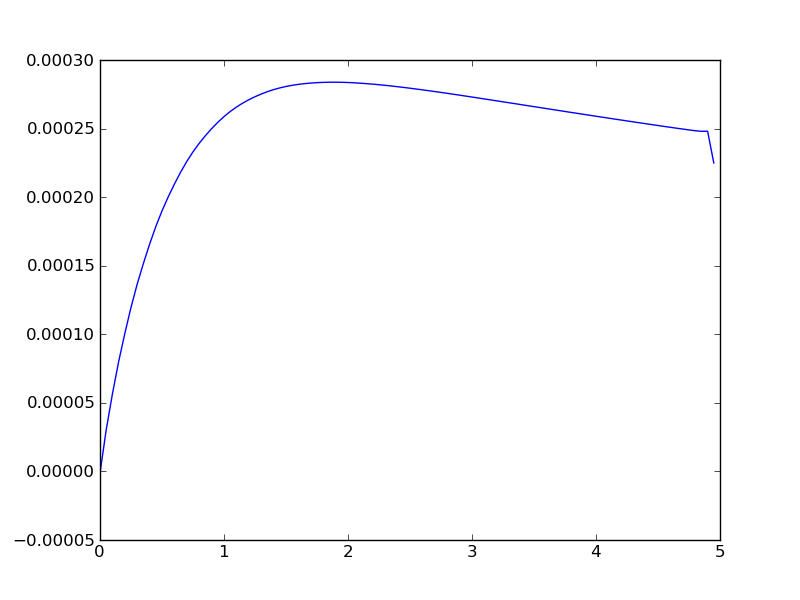
\includegraphics[width=\linewidth]{./images/al/group_39_moment_30}
\caption{Moment $P_5^0$ of the flux in the last electron group}
\end{minipage}
\end{figure}

\begin{figure}[H]
\begin{minipage}[b]{0.42\linewidth}
\centering
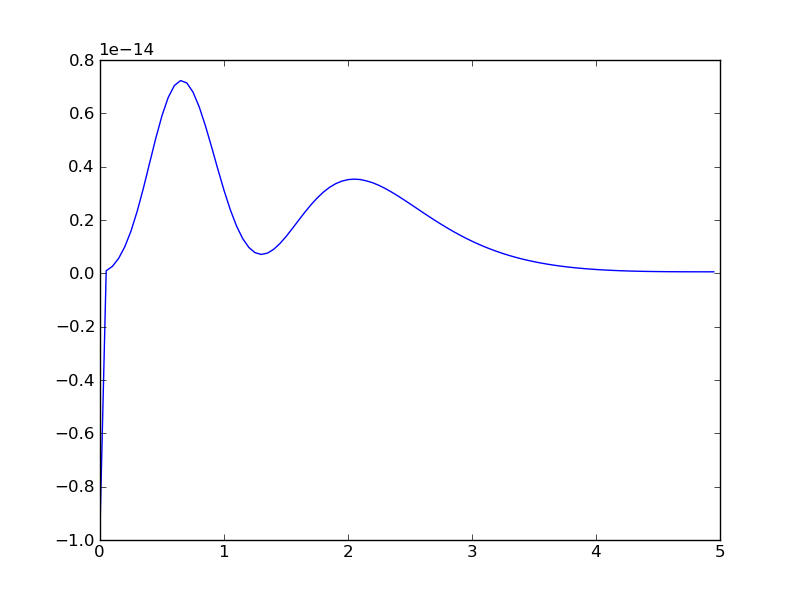
\includegraphics[width=\linewidth]{./images/al/group_0_moment_142}
\caption{Moment $P_{11}^0$ of the flux in the first photon group}
\end{minipage}
\hspace{0.5cm}
\begin{minipage}[b]{0.42\linewidth}
\centering
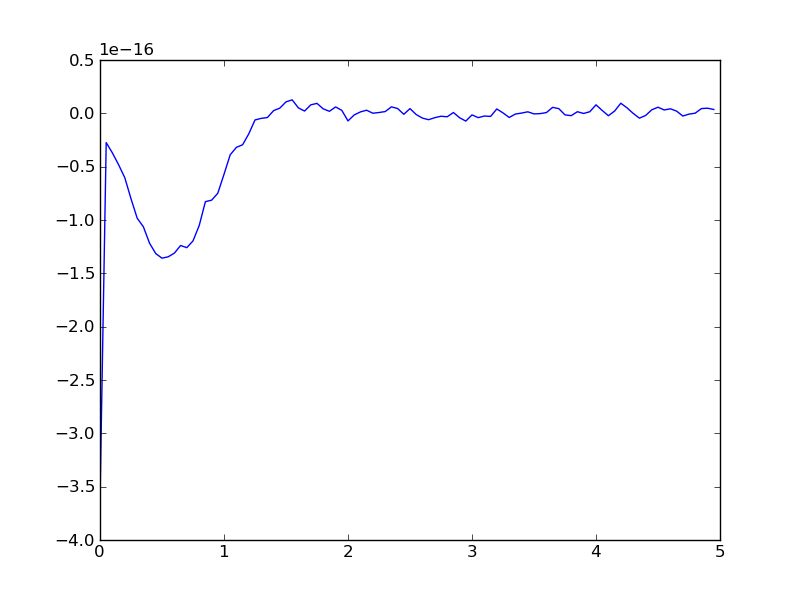
\includegraphics[width=\linewidth]{./images/al/group_39_moment_142}
\caption{Moment $P_5^0$ of the flux in the last electron group}
\end{minipage}
\end{figure}

\subsection{Gold}
The setup of this problem is the same as for the previous simulations but the
medium considered here is gold. In the next table, we provide the dose computed every centimeter 
using a different scattering order :
\begin{table}[H]
\begin{center}
\caption{Dose in $\frac{MeV}{g}$ for different scattering orders}
\begin{tabular}{|c|c|c|c|c|c|}
\hline
Position & ONELD &  order = 11 & order = 9 & order = 7 & order = 5 \\
\hline
0 & 0.11675 & 0.097168 & 0.097155 & 0.097073 & 0.097326 \\
1 & 0.41799 & 0.420905 & 0.420871 & 0.420988 & 0.421102 \\
2 & 0.16284 & 0.164953 & 0.164946 & 0.165017 & 0.164605 \\
3 & 0.06407 & 0.065297 & 0.065300 & 0.065292 & 0.065214 \\
4 & 0.02566 & 0.026303 & 0.026304 & 0.026295 & 0.026318 \\
5 & 0.00847 & 0.006082 & 0.006083 & 0.006075 & 0.006112 \\
\hline
\end{tabular}
\end{center}
\end{table}                
We can see that there is no need to use the full order to solve the problem.
The differences between the order 5 and order 11 are small. We do not have the
results for the order 13 yet but we do not expect to see the results to be
very different from the order 11. The difference between the order 11 and ONELD
is about 2\% in the middle of the domain. The difference is larger on the
boundary of the domain due to the interpolation of the ONELD results.

